\documentclass[twoside]{amsart}
\usepackage{amsmath,amsthm,amsfonts,amssymb}
\usepackage{color}
\usepackage[pagebackref,colorlinks,citecolor=blue,linkcolor=blue,urlcolor=blue,filecolor=blue]{hyperref}
\usepackage{tikz}
\usetikzlibrary{shapes.geometric}
\tikzset{
v/.style={draw, fill, circle, minimum size=1.5mm, inner sep=0},
b/.style={draw , regular polygon,regular polygon sides=4, minimum size=1.5mm, inner sep=.5mm},
e/.style={very thick},
vs/.style={draw, fill, circle, minimum size=1mm, inner sep=0},
bs/.style={draw,  regular polygon,regular polygon sides=4, minimum size=2mm, inner sep=0mm},
es/.style={thick}
}
\usetikzlibrary{arrows,matrix,positioning}

\begin{document}

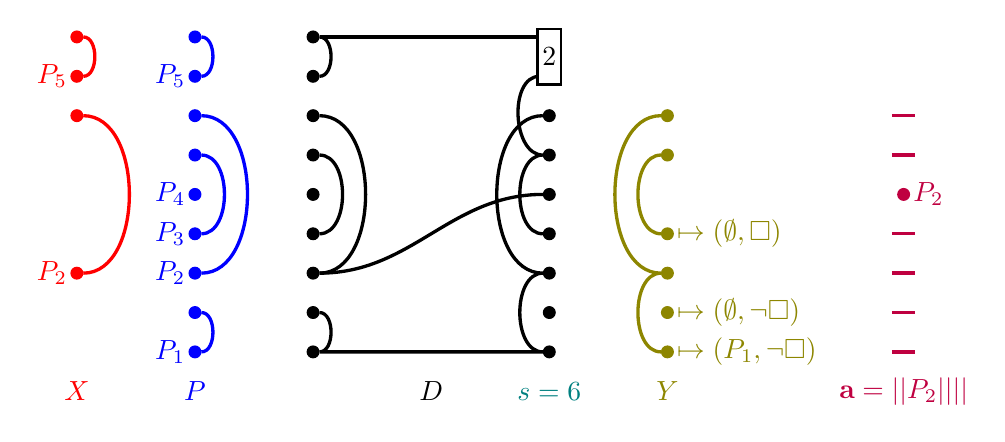
\begin{tikzpicture}[x=1.5cm,y=-.5cm,baseline=-2.05cm]
    
        \node[v] (a1) at (0,0) {};
        \node[v] (a2) at (0,1) {};
        \node[v] (a3) at (0,2) {};
        \node[v] (a4) at (0,3) {};
        \node[v] (a5) at (0,4) {};
        \node[v] (a6) at (0,5) {};
        \node[v] (a7) at (0,6) {};
        \node[v] (a8) at (0,7) {};
        \node[v] (a9) at (0,8) {};

        \node[v,blue] (c1) at (-1,0) {};
        \node[v,blue] (c2) at (-1,1) {}; 
        \node[v,blue] (c3) at (-1,2) {};
        \node[v,blue] (c4) at (-1,3) {}; 
        \node[v,blue] (c5) at (-1,4) {};
        \node[v,blue] (c6) at (-1,5) {}; 
        \node[v,blue] (c7) at (-1,6) {};
        \node[v,blue] (c8) at (-1,7) {}; 
        \node[v,blue] (c9) at (-1,8) {};

        \node[v,red] (d1) at (-2,0) {};
        \node[v,red] (d2) at (-2,1) {}; 
        \node[v,red] (d3) at (-2,2) {};
        \node[v,red] (d7) at (-2,6) {};
        
        \node (b1) at (2,0) {};
        \node (b2) at (2,1) {};
        \node[v] (b3) at (2,2) {};
        \node[v] (b4) at (2,3) {};
        \node[v] (b5) at (2,4) {};
        \node[v] (b6) at (2,5) {};
        \node[v] (b7) at (2,6) {};
        \node[v] (b8) at (2,7) {};
        \node[v] (b9) at (2,8) {};

        
        \node[v,olive] (e3) at (3,2) {};
        \node[v,olive] (e4) at (3,3) {};
        \node[v,olive] (e6) at (3,5) {};
        \node[v,olive] (e7) at (3,6) {};
        \node[v,olive] (e8) at (3,7) {};
        \node[v,olive] (e9) at (3,8) {};
        
        \draw[e] (a1) to[out=0, in=180] (b1);      
        \draw[e] (a7) to[out=0, in=180] (b5);
        \draw[e] (a1) to[out=0, in=0] (a2);
        \draw[e] (a8) to[out=0, in=0] (a9) to[out=0, in=180] (b9) to[out=180, in=180] (b7) to[out=180, in=180] (b3);
        \draw[e] (a3) to[out=0, in=0]   (a7);
        \draw[e] (a4) to[out=0, in=0]   (a6);
        \draw[e] (b2) to[out=180, in=180](b4) to[out=180, in=180] (b6);
        
        \draw[fill=white, line width=1] (1.9,-0.2) rectangle (2.1,1.2);
        \node at (2,0.5) {$2$};
        
        \draw[e,blue] (c1) to[out=0, in=0] (c2);
        \node[left,blue] at (c9) {$P_1$};
        \node[left,blue] at (c7) {$P_2$};
        \node[left,blue] at (c6) {$P_3$};
        \node[left,blue] at (c5) {$P_4$};
        \node[left,blue] at (c2) {$P_5$};
        \draw[e,blue] (c8) to[out=0, in=0] (c9);
        \draw[e,blue] (c3) to[out=0, in=0]   (c7);
        \draw[e,blue] (c4) to[out=0, in=0]   (c6);
        
        \draw[e,red] (d1) to[out=0, in=0] (d2);
        \node[left,red] at (d7) {$P_2$};
        \node[left,red] at (d2) {$P_5$};
        \draw[e,red] (d3) to[out=0, in=0]   (d7);
        
        \draw[e,olive] (e9) to[out=180, in=180] (e7) to[out=180, in=180] (e3);
        \draw[e,olive] (e4) to[out=180, in=180] (e6);
        \node[right,olive] at (e6) {$\mapsto(\emptyset, \square)$};
        \node[right,olive] at (e9) {$\mapsto(P_1, \neg\square)$};
        \node[right,olive] at (e8) {$\mapsto(\emptyset, \neg\square)$};
    
       
        \draw[e,purple] (4.9,2) to (5.1,2);
        \draw[e,purple] (4.9,3) to (5.1,3);
        \node[v,purple] at (5,4) {};
        \node[right,purple] at (5,4) {$P_2$};
        \draw[e,purple] (4.9,5) to (5.1,5);
        \draw[e,purple] (4.9,6) to (5.1,6);
        \draw[e,purple] (4.9,7) to (5.1,7);
        \draw[e,purple] (4.9,8) to (5.1,8);
        
        \node[red] at (-2,9) {$X$};
        \node[blue] at (-1,9) {$P$};
        \node at (1,9) {$D$};
        \node[teal] at (2,9) {$s=6$};
        \node[olive] at (3,9) {$Y$};
        \node[purple] at (5,9) {$\mathbf{a}=||P_2||||$};
    \end{tikzpicture}

\end{document}